%!TEX root = ../../../adrien_gomar_phd.tex
\chapter{Preliminary validations of the harmonic balance approach}
\label{cha:validation_hb}

\chabstract{In this chapter the mono- and
multi-frequential harmonic balance approaches
are validated. In this aim, two model problems are used.
Firstly, the harmonic balance method is applied to the linear advection equation 
supplemented with unsteady boundary conditions 
of different frequency content. Mono- and multi-frequential
unsteady signals are injected and compared to
exact solutions. The spectral accuracy of the method is verified.
Moreover, the ability of the multi-frequential
approach to capture signal composed of segregated frequencies
is underlined. Based on these results, the aeroelasticity
of contra-rotating open rotors is put into perspectives.
Secondly, the multi-frequential approach is assessed for
a channel flow problem solved using the \emph{elsA}~\cite{Cambier2013}
CFD code within the Navier--Stokes equations framework. The results
are shown to be superimposed with a classical time-marching solution.}

\newpage

\section{Linear advection of a periodic signal}
\label{sec:linear}
%!TEX root = ../../../adrien_gomar_phd.tex

\subsection{Presentation of the test case}
\label{sec:presentation_advection}

To validate the harmonic balance approach within a 
linear framework, the resolution of the
advection equation is considered. It is defined as
\begin{equation}
  \label{eq:convection}
  \frac{\partial u}{\partial t} + c \frac{\partial u}{\partial x} = 0,
\end{equation}
with the constant advection speed $c$ assumed as positive. 
The equation is solved in the domain $x \in [0, L_x]$. 
Periodic perturbations of different shapes are imposed at the left boundary
\begin{equation}
   u(0, t) = u_l (t),
\end{equation}
where $u_l$ is a periodic function of period $T=L_x/c$.
These perturbations are advected across the computational 
domain and leave from the right boundary. After a transient of time length $T_{trans}=L_x/c$, 
the solution at any point $x$ in the space domain achieves a periodic state. 
The exact solution for this periodic state is a periodic function of the form
\begin{equation}
    u_{ex}(x,t)=u_l(x/c+t).
\end{equation}
For simplicity, $L_x$ and $c$ are taken as unity.

\subsection{Numerical setup}

The space derivative is discretized by means of a centered 
fourth-order finite-difference scheme on a uniform Cartesian mesh
\begin{equation}
    \frac{\partial u}{\partial x} (x = x^i, \replaced{\tau=\tau_q}{t=t_q}) =
    \frac{-u^{i+2}_{q} + 8 u^{i+1}_{q} - 8 u^{i-1}_{q} + u^{i-2}_{q}}{12\Delta x}
    + \mathcal{O} (\Delta x^4),
    \label{eq:convection_center4}
\end{equation}
A very fine space step is used ($\Delta x=5\e{-4}$) in order to rule 
out spatial approximation errors. This corresponds to $2,000$ grid points
in the domain. 
The solution at the last mesh 
point on the right of the domain is extrapolated 
from the inside. To this aim, a standard second-order 
and a first-order upwind discretization schemes
are used to approximate the space derivative at 
the last two mesh points on the right, respectively
\begin{equation}
    \begin{split}
        &\frac{\partial u}{\partial x} (x = x^{m-1}, \replaced{\tau=\tau_q}{t=t_q}) =
            \frac{3 u^{m-1}_{q} - 4 u^{m-2}_{q} + u^{m-3}_{q}}{2\Delta x} + \mathcal{O} (\Delta x^2), \\
        &\frac{\partial u}{\partial x} (x = x^m, \replaced{\tau=\tau_q}{t=t_q}) = 
            \frac{u^{m}_{q} - u^{m-1}_{q}}{\Delta x} + \mathcal{O} (\Delta x),
    \end{split}
\label{eq:upwind_scheme}
\end{equation}
where $m$ is the total number of grid points.

Time-discretization is achieved 
through the HB method (described in Sec.~\ref{sec:sm_hb})
with a standard four-step Runge-Kutta method~\cite{Jameson1981}
used to pseudo-time 
march the HB equations to the steady-state.
The $k\textsuperscript{th}$ step is evaluated by
\begin{equation}
    u_k = u_q - \alpha_k \replaced{\Delta \tau}{\Delta t} \left [ 
          c \frac{\partial u_{k-1}}{\partial x} 
          (\replaced{\tau=\tau_q}{t=t_q} + \alpha_{k-1} \replaced{\Delta \tau}{\Delta t})
          + D_t(u_k)
          \right],
    \label{eq:convection_rk4}
\end{equation}
where $\alpha_0 = 0$, $\alpha_1 = 1/4$, 
$\alpha_2 = 1/3$, $\alpha_3 = 1/2$, $\alpha_4 = 1$. 
The HB source term $D_t(u_k)$ is computed 
using Eq.~\eqref{eq:sm_multi_spectral_operator}.

\replaced{The CFL number in pseudo-time is set to 1 
to ensure the stability of the explicit time-marching scheme
which sets the time step.
For stability reasons, this time step
is modified~\cite{Weide2005} to take into account
the additional source term
\begin{equation}
  \label{eq:stabdeltat}
  \Delta\tau = \text{CFL} \frac{\Delta x}{c + \omega N \Delta x}.
\end{equation}
The extra term $\omega N \Delta x$ is added 
to the advection velocity $c$ to
restrict the time step.  Equation~\eqref{eq:stabdeltat} implies that a
high frequency and/or a high number of harmonics~$N$ can considerably
restrict the time step, especially for explicit Runge Kutta time
integration scheme, as mentioned in~\cite{Hall2002}. Moreover, for 
the multi-frequential
computations, the extra term $\omega N \Delta x$ is
replaced by $\omega_N \Delta x$, where $\omega_N$ denotes
the largest angular frequency.}{
The CFL number in pseudo-time is set to 1 
to ensure stability of the explicit time-marching scheme.}

\subsection{Validation of the mono-frequential approach}
\label{sec:sum_sine}

A perturbation 
in the form of a finite sum of sine functions, similar to the one used
in Sec.~\ref{sec:hb_operator},
is applied at the left boundary
\begin{equation}
    u_l(t) = \cos(\omega t) + \sin(2 \omega t) +
    \cos(3 \omega t) + \sin(4 \omega t) + \cos(5 \omega t).
    \label{eq:sum_injected_fct}
\end{equation}
Harmonic balance computations are run with 1 to 10~harmonics.
For each computation, we show spatial distributions of the solution
at three time instants, namely $t=0$, $t=T/3$ and $t=2T/3$.
Since these instants are not necessarily used in the HB discretization,
a temporal interpolation is performed.
To do so, the frequency content of the HB solution is used
together with an inverse Fourier transform on the time-vector
$[0, T/3, 2T/3]$.
Figure~\ref{fig:inj_sine_results} depicts the results of HB computations
using 1 to 5~harmonics. The analytical solution is also reported for comparison.
\begin{figure}[htp]
  \centering
  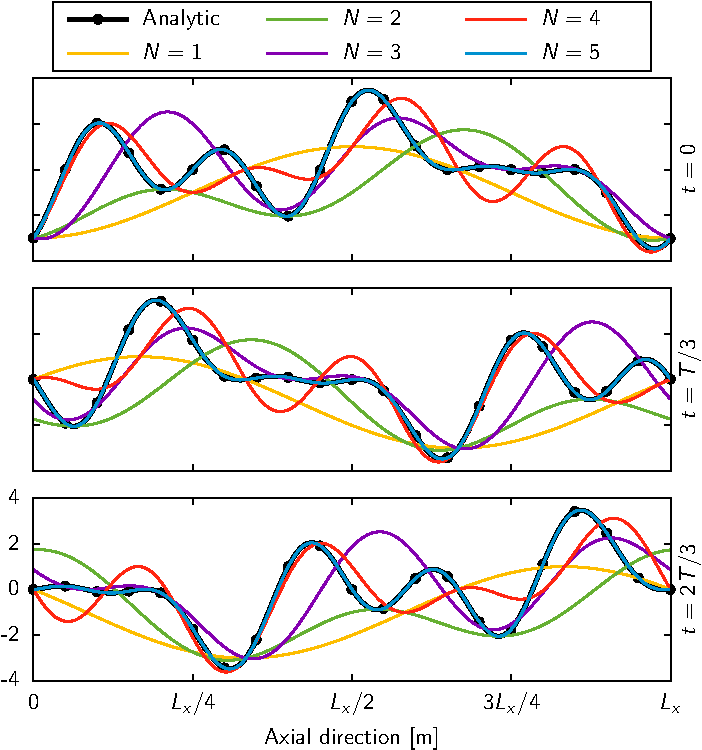
\includegraphics[width=.5\textwidth]{convection_sin.pdf}
  \caption{Linear advection of a sum of sine functions: 
  numerical solutions at different time instants for different numbers of harmonics.}
  \label{fig:inj_sine_results}
\end{figure}


The accuracy of the solution 
improves with the number of harmonics,
until it reaches the frequency content
of the injected signal, \emph{i.e.} 5~harmonics.
For higher sampling levels, the results of HB computations are
superimposed with the analytical solution, validating the current approach.

The $\mathcal{L}_2$-norm of the error 
in time is computed over all the time instants
at each grid point over the domain.
Then, the average in space is computed.
The error is shown as a function of the number of harmonics
in Figure~\ref{fig:conv_sum_sine}. Two results are displayed:
one for the reference mesh (2,000 grid points) and one for
a refined mesh (4,000 grid points).
\begin{figure}[htp]
  \centering
  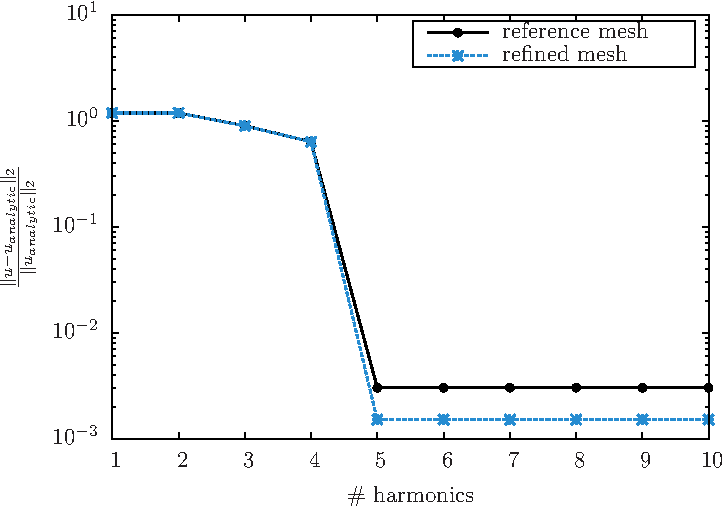
\includegraphics[width=.5\textwidth]{convection_sin_error.pdf}
  \caption{Linear advection of a sum of sine functions: convergence of the HB method error.}
  \label{fig:conv_sum_sine}
\end{figure}
The convergence of the HB computations is slow  for
$N \leq 4$. However, when the number of harmonics composing
the injected function is reached ($N=5$), the error is minimum and computing
more harmonics does not change the error. As introduced in 
Sec.~\ref{sec:spectral_accuracy},
the convergence rate 
of Fourier-based time methods is inherently linked to the spectrum of the
temporal phenomenon that one wants to capture. This property is still
seen when solving the linear advection equation.
Here a finite discrete spectrum composed of only five harmonics
is imposed.
The value of the plateau obtained 
after $N=5$ is representative of the error introduced by the different
discretizations. In fact, refining the mesh changes this value
without modifying the error levels of the lower harmonics points
as indicated by Figure~\ref{fig:conv_sum_sine}.

The temporal discrete Fourier transform
of the computational results is compared to the
analytical results in Figure~\ref{fig:dft_sin}.
\begin{figure}[htp]
  \centering
  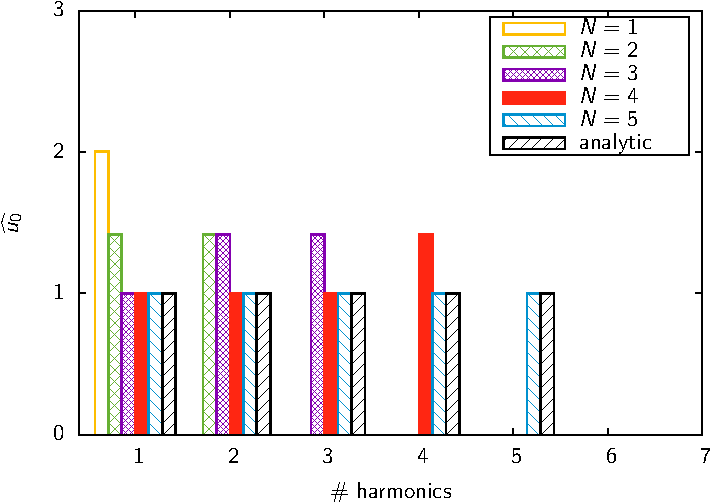
\includegraphics[width=.5\textwidth]{convection_sin_dft.pdf}
  \caption{Linear advection of a sum of sine functions: 
  discrete Fourier transform.}
  \label{fig:dft_sin}
\end{figure}
When the number of harmonics grows in the spectral computations,
the Fourier transform gets closer to the analytical solution.
When the whole frequency content of the injected 
function is contained in the HB solution, 
the numerical results are superimposed with the analytical ones.
For intermediate sampling frequencies, as for 
instance the three-harmonics HB computation, 
the resolved harmonics have higher amplitudes 
than the exact one, since they compensate for harmonics that are not resolved.

When the number of harmonics composing the spectrum of the
computed signal is reached, the computational results are superposed
with the analytical ones, namely we obtain spectral accuracy.
This is the main advantage of Fourier-based time methods: when the
signal has a narrow spectrum, as it is the case for the sum
of sine function used here, the
convergence can be very fast compared to a classical time-marching scheme
as only a few number of time instants is necessary to retrieve the
unsteadiness.


\subsection{Validation of the multi-frequential approach}

In Section~\ref{sec:sm_hb_multi}, the multi-frequential harmonic
balance approach has been presented. In this method,
the frequencies can be chosen arbitrarily. This becomes particularly
interesting when dealing with signal/flow field composed of segregated
frequencies. To emphasize that, let us consider the linear advection problem
with a perturbation 
in the form of a sum of two sine functions,
applied at the left boundary
\begin{equation}
    u_l(t) = \sin(\omega t) + \sin(22 \omega t).
    \label{eq:multifreq_inj_func}
\end{equation}

\subsubsection{Using a mono-frequential approach}

Obviously, computing the advection of such a perturbation using
a classical time-marching scheme would require to discretize the
smaller period. The largest frequency
(here $f_2 = 22$~Hz) acts as a bottleneck as the time-step will be chosen
according to this frequency. The cost scales thus with the ratio of $f_2 / f_1$.

This holds true when computing the solution using the mono-frequential
harmonic balance approach. In fact, the frequencies can not be chosen arbitrarily.
Therefore, to compute such a configuration, a $N=22$ harmonic computation
will be needed to be spectral accurate. To emphasize that, mono-frequential
HB computations are run with 1 to 25~harmonics.
As made previously, 
for 6 chosen computations of the~25 computations, 
we show spatial distributions of the solution
at three time instants, namely, $t=0$, $t=T/3$ and $t=2T/3$.
It is shown in Figure~\ref{fig:inj_multifreq_tsm}.
\begin{figure}[htp]
  \centering
  \subfigure[$N=1$]{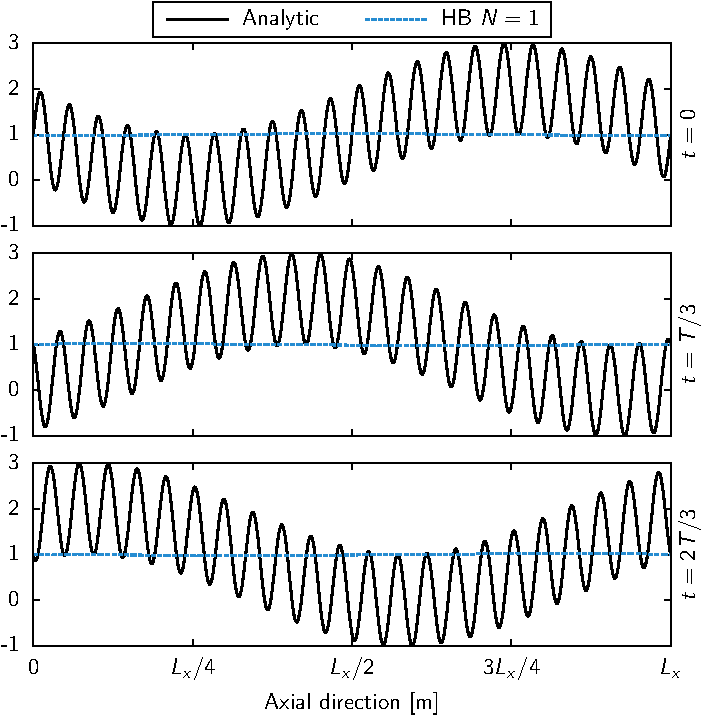
\includegraphics[width=.35\textwidth]{convection_multifreq_tsm_N1.pdf}}
  \subfigure[$N=5$]{
    \label{fig:convection_multifreq_tsm_N5}
    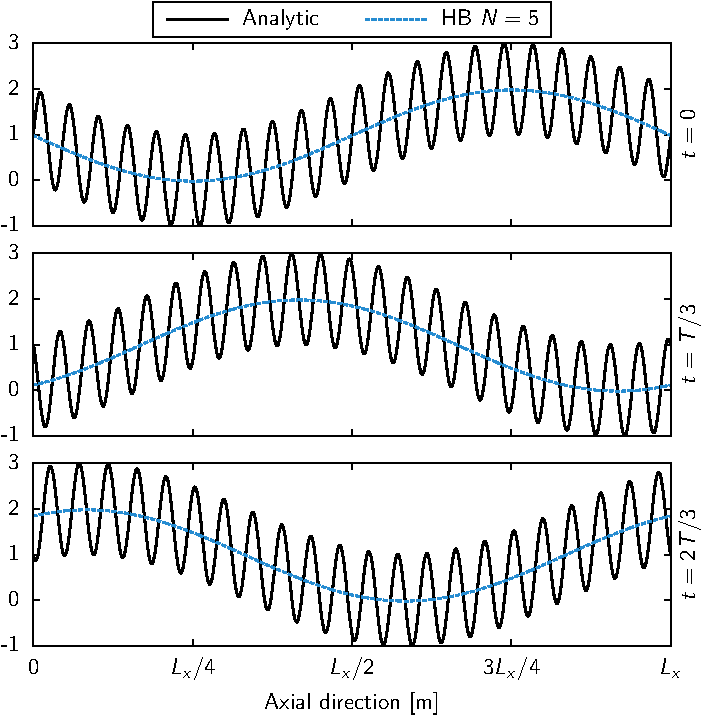
\includegraphics[width=.35\textwidth]{convection_multifreq_tsm_N5.pdf}}
  \subfigure[$N=11$]{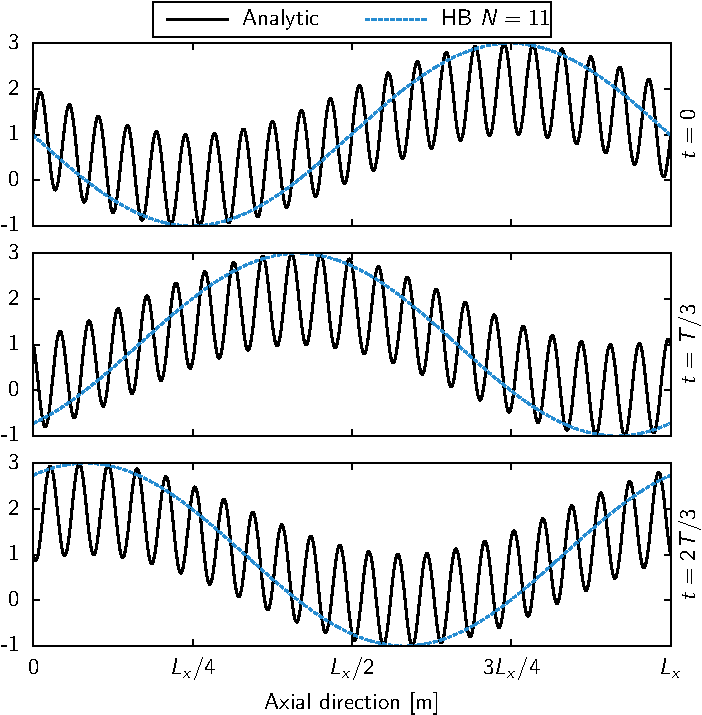
\includegraphics[width=.35\textwidth]{convection_multifreq_tsm_N11.pdf}}
  \subfigure[$N=16$]{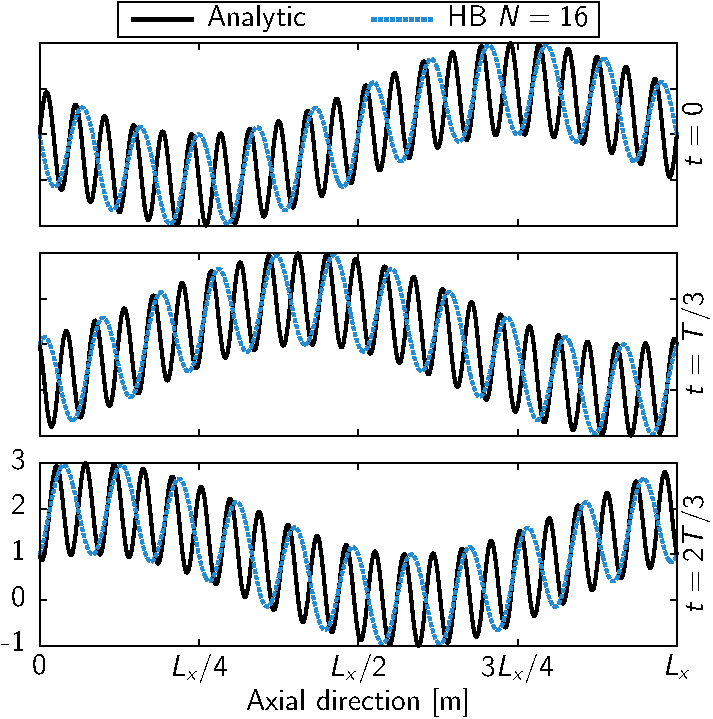
\includegraphics[width=.35\textwidth]{convection_multifreq_tsm_N16.pdf}}
  \subfigure[$N=22$]{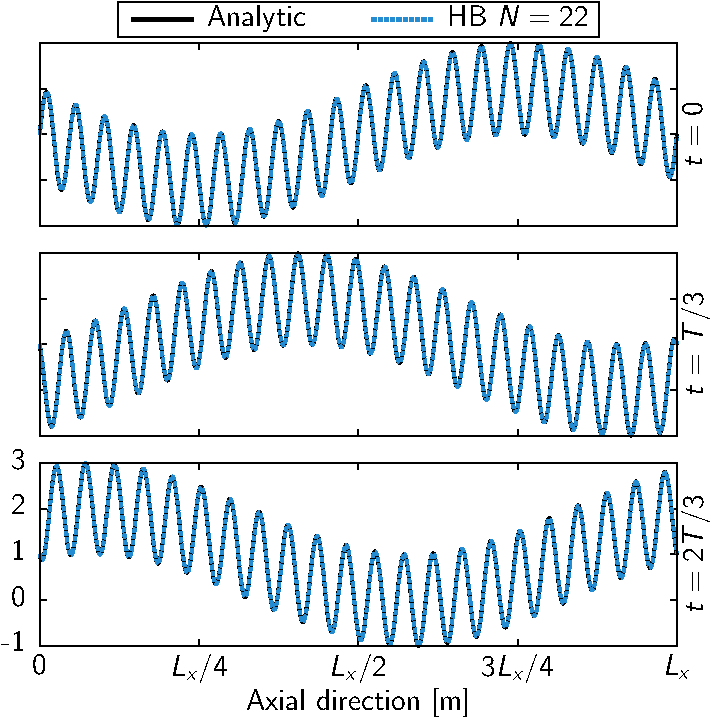
\includegraphics[width=.35\textwidth]{convection_multifreq_tsm_N22.pdf}}
  \subfigure[$N=23$]{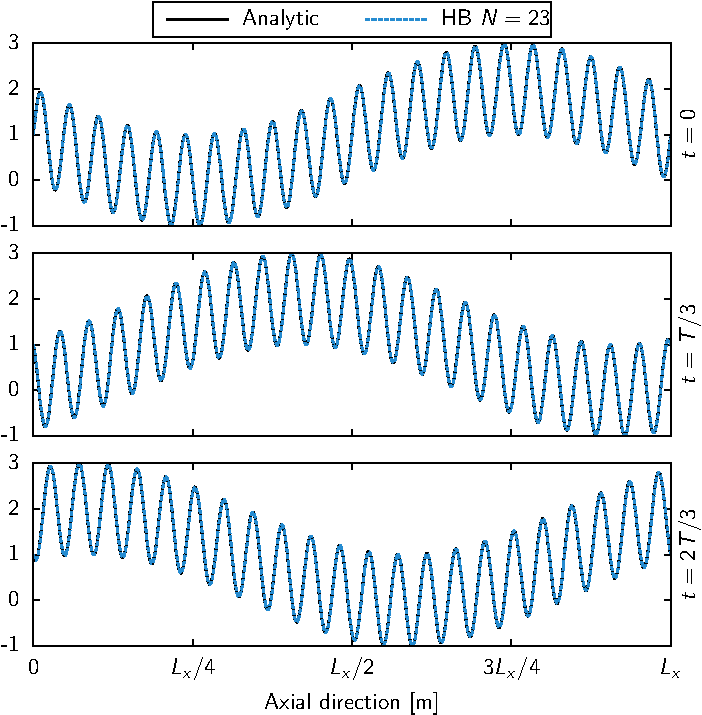
\includegraphics[width=.35\textwidth]{convection_multifreq_tsm_N23.pdf}}
  \caption{Linear advection of a sum of two segregated sine functions: 
  numerical solutions at different time instants for different numbers of harmonics.}
  \label{fig:inj_multifreq_tsm}
\end{figure}
Again, the accuracy in capturing the injected function
improves with the number of harmonics,
until it reaches the frequency content
of the injected signal, \emph{i.e.} 22~harmonics.
After that, the results of the HB computations are
superimposed with the analytical solution. 
The problem, with such a segregation of frequencies, is that 
the mono-frequential version suffers from the same
problems as a classical time-marching scheme in terms of 
computational cost.

To quantitatively analyze the results,
the discrete $\mathcal{L}_2$-norm of the error 
is shown in Figure~\ref{fig:conv_multifreq_tsm} for the
mono-frequential HB computations ranging from 1 to~25
harmonics.
\begin{figure}[htp]
  \centering
  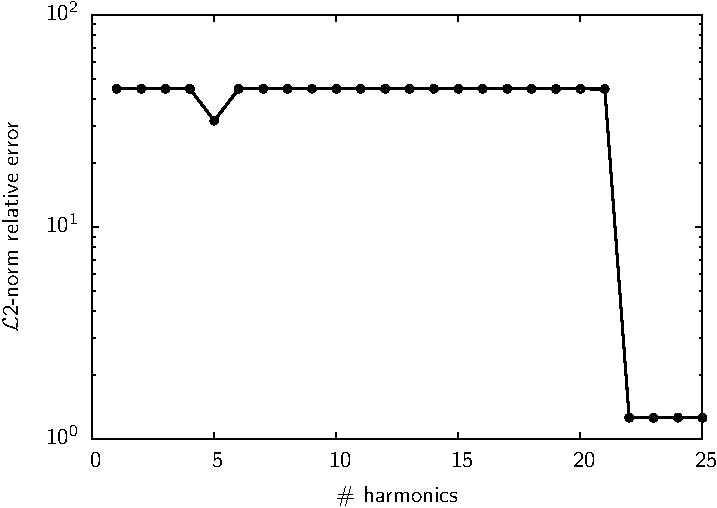
\includegraphics[width=.5\textwidth]{convection_multifreq_error.pdf}
  \caption{Linear advection of a sum of two segregated sine functions: convergence of the mono-frequential HB method error.}
  \label{fig:conv_multifreq_tsm}
\end{figure}
When the number of harmonics
used to compute the solution is higher than the content of the spectrum,
the error decreases drastically. The spectral accuracy is retrieved
but only starting at $N=22$.
In fact, similar as in Sec.~\ref{sec:sum_sine},
the injected function is indefinitely differential and periodic
yielding an infinite convergence slope. We can observe a slight local convergence
for the $N=5$ harmonics HB computation. This is due to the fortunate 
capture of the low-frequency pattern of the injected function
as shown in Figure~\ref{fig:convection_multifreq_tsm_N5}.

\subsubsection{Using a multi-frequential approach}

One of the advantage of the multi-frequential HB method, 
introduced in Sec.~\ref{sec:sm_hb_multi}
and used in this work, is that it can take arbitrary frequencies into account.
In the case of an injected signal with a large frequency segregation, the
benefit might be tremendous. Let us consider again the signal defined in 
Eq.~\eqref{eq:multifreq_inj_func} and compute one HB simulation using 
$f_1=1$~Hz and $f_2=22$~Hz as input frequencies. This gives a computation
of two coupled calculation
that is nine times faster than the $N=22$ converged mono-frequential
HB computation. \added{In fact, the cost of a $N=22$ computation scales with
$2 \times 22 + 1=45$ (see Sec.~\ref{sec:sm_hb_cost}), 
while a $N=2$ computation scales with $2 \times 2 + 1=5$
which explains the nine factor.}

Again
we show spatial distributions of the solution
at three time instants, namely $t=0$, $t=T/3$ and $t=2T/3$
in Figure~\ref{fig:inj_multifreq_hb}.
\begin{figure}[htp]
  \centering
  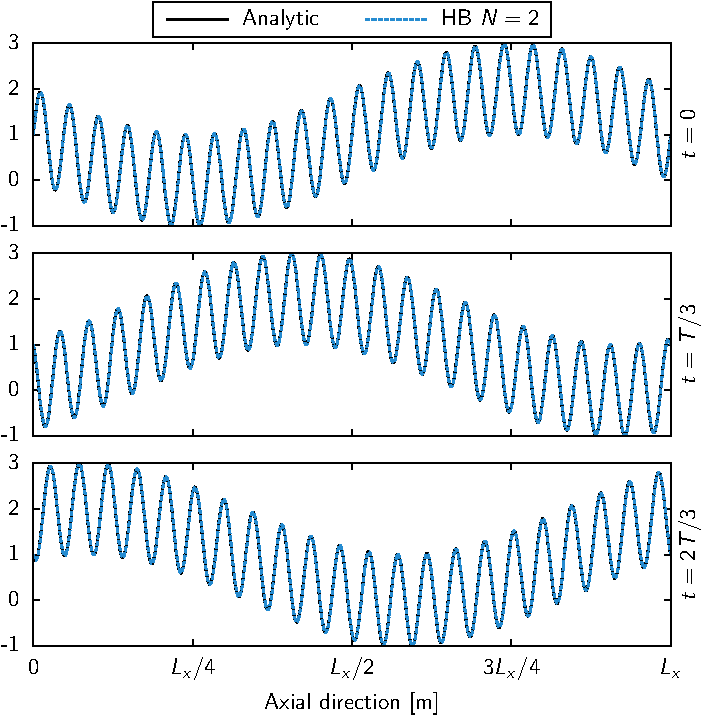
\includegraphics[width=.5\textwidth]{convection_multifreq_hbt_N2.pdf}
  \caption{Linear advection of a sum of two segregated sine functions: 
  numerical solutions at different time instants for different numbers of harmonics using the
  multi-frequential harmonic balance method.}
  \label{fig:inj_multifreq_hb}
\end{figure}
With only two input frequencies, the multi-frequential
HB solution is superimposed with the analytical solution.
Moreover, the $\mathcal{L}2$-norm of the error is 
exactly the same as the one of the $N=22$ mono-frequential
approach.

This validates the multi-frequential approach 
used along with segregated frequencies which is 
the case of contra-rotating open rotor aeroelasticity.


\section{Application to a non-linear system of equations}
\label{sec:non_linear}
%!TEX root = ../../../adrien_gomar_phd.tex
\subsection{Presentation of the case}
\label{sec:channel_flow_problem}

The second toy problem considered represents a 2D channel 
with a constant left injection at 
a transonic Mach number ($M=0.7$)
supplemented with a time-varying unsteady back pressure.
As the pressure is oscillating at the outlet, the imposed unsteady pressure
fluctuations travel within the flow at the velocity 
$u + c$ and $u - c$, where $u$ denotes 
the local flow velocity and $c$ the speed of sound.
Since the pressure waves are generated at the outlet, only
the $u-c$ waves are seen, resulting in pressure waves propagating
upstream of the channel. The axial length of the channel is $L_x = 100$~m
and $L_y = 1$~m in the transverse direction.
Figure~\ref{fig:canal_principle} shows a sketch
of the considered channel flow problem.
\begin{figure}[htp]
  \centering
  \includegraphics*[width=0.65\textwidth]{channel_sketch.pdf}
  \caption{Sketch of the channel flow problem.}
  \label{fig:canal_principle}
\end{figure}

\citet{Merkle1987} give an analytical solution
for incompressible flows with small pressure fluctuations, assuming
thus a linear unsteady flow.
However, this toy problem is set up to highlight the properties
of the harmonic balance in a non-linear framework which is not
the hypothesis of \citet{Merkle1987}. Nevertheless, to give confidence
in our forthcoming results for this toy problem,
this last will be validated below against a classical time-marching scheme
in Sec.~\ref{sec:channel_multifreq}.

\subsection{Numerical setup}

% mesh presentation
The mesh consists of 997~points along the axial direction and 9~in the
transverse one, which corresponds to equal spacings in both
directions. 

% boundary conditions
The boundary conditions are: (i)~a constant injection condition for the inlet
where the total pressure $p_{i_0}$ and enthalpy $h_{i_0}$ are set,
(ii)~symmetric conditions for the upper and lower bounds as the flow
is assumed to be symmetric in the transverse direction, and (iii)~a
fluctuating static pressure imposed at the outlet:
\begin{equation}
  p_{s_1}(t) = \overline{p}_{s_1} \left[1 + a_1 \sin(2 \pi f_1 t) +
    a_2 \sin(2 \pi f_2 t) \right],
  \label{eq:outlet_canal}
\end{equation}
where $\overline{p}_{s_1}$ is the temporal average static pressure, $a_n$ the
amplitude of the $n$\textsuperscript{th} mode and $f_n$ its
frequency. Only two modes ($f_1$, $f_2$) are injected
but due to the non-linearity of the Navier--Stokes equations,
new frequency combinations rise.
The mean velocity of the flow is imposed through a
static pressure condition $\overline{p}_{s_1}$ at the outlet:
\begin{equation}
    \overline{p}_{s_1} = \frac{p_{i_0}}{\left(1 + 
    \frac{\gamma - 1}{2} M_{0}^2 \right) ^ {\frac{\gamma}{ \gamma - 1}}} ,
\end{equation}
the mean velocity is thus set by imposing the
inlet target mean Mach number value $M_{0}$.
We assume here that the flow is isentropic as no
geometrical object disturbes the flow field.

% solver
The \textit{elsA}~\cite{Cambier2013} CFD code developed by ONERA
is used to solve this toy problem. In fact, 
the aim of this toy problem is 
to use the same
solver as the one used in the application part of this
thesis so that the results shown here can be directly
transposed. 
This code solves the RANS equations using a cell-centered
approach on multi-blocks structured meshes.
Several time-integration schemes
are available, in particular the Dual Time-Stepping~\cite{Jameson1981} (DTS)
as well as the time-domain harmonic 
balance method implemented by \citet{JSicot2008} for the mono-frequential
formulation and extended by \citet{JGuedeney2013} to multi-frequential flows. 


% numerical schemes
The present configuration is turbulent as the Reynolds number based on the
inlet flow velocity and the axial length of the channel is about $R_e
\approx 2.0 \times 10^9$. To this aim, turbulence is modeled using the
one-equation model of \citet{Spalart1992}.
Roe's scheme~\cite{Roe1981} along with a third-order MUSCL extrapolation 
is used for the spatial discretization of
the convective fluxes. An implicit backward Euler scheme is used
to march the HB equations in pseudo-time.

\subsection{Validation of the multi-frequential approach}
\label{sec:channel_multifreq}

As no analytical solution is available for this case, we propose
now to validate the channel flow toy problem within a HB framework
in order to have confidence in the forthcoming results on this
toy problem.
To do so, two non-harmonically related
frequencies are chosen as input for the outlet boundary condition:
$f_1 = 3$~Hz and $f_2 = 17$~Hz.

The classical DTS time-marching scheme is taken for comparison.
Convergence in time discretization is obtained after 20~periods using
160~instants per almost-period. Since the frequencies are integers and
coprime, the period is $T=1$~s.  Iterative convergence for the
inner loop is considered achieved when the normalized residuals drop
by $10^{-2}$ within a maximum of 50~sub-iterations.

The results obtained with the DTS scheme are compared to the HB
results for pressure waves amplitudes of $a = a_1 = a_2 = 0.001$
(see Eq.~\eqref{eq:outlet_canal}).  The
transient of the DTS computation is shown in
Fig.~\ref{fig:canal2_transient}, illustrating the wave propagation
with a slight attenuation of the high-frequency waves.
\begin{figure}[htp]
  \centering
  \includegraphics*[width=.5\linewidth]{CANAL2_TRANSIENT_PPT.pdf}
  \caption{DTS computation: transient propagation of the pressure waves.}
  \label{fig:canal2_transient}
\end{figure}

Due to the non-linearity of the Navier--Stokes equation, the two frequencies
$f_1$ and $f_2$ give rise to linear combinations of them.
Therefore, the results are analyzed for frequencies $1<f< 40~\textrm{Hz}$ and the
dominant frequencies (the one that have the highest amplitudes) are
set for the HB computation.  To do so, pressure signals are probed
upstream, in the middle and downstream of the channel at
$x=[25~\textrm{m}, 50~\textrm{m}, 75~\textrm{m}]$ and $y=0.5$~m
respectively.  The spectrum of the aforementioned unsteady pressure
signals, obtained with a Fourier Transform is plotted in
Fig.~\ref{fig:canal2_dts_fft}.  The labeled frequencies are the
dominant ones, as for each probe, these have a high amplitude. Those
nine frequencies are thus selected as input frequencies for the HB computation.
\begin{figure}[htp]
  \centering
  \includegraphics*[width=.5\linewidth]{channel_dts_fft_plus_sketch.pdf}
  \caption{Spectrum of pressure signals.}
  \label{fig:canal2_dts_fft}
\end{figure}

The HB computation using the previously mentioned frequencies is
run and a discrete Fourier transform is computed at several axis positions
in the middle of the channel ($y=0.5$~m). 
This is the same post-processing as done previously to retrieve 
Fig.~\ref{fig:canal2_dts_fft}, but for all axial grid points.

Figure~\ref{fig:canal2_validation_hbt_gear_amp_vs_axis}
shows the results for the frequencies that have been set for the HB computation.
The overall agreement between the DTS and the HB is fair.  
Some local discrepancies can be
observed upstream for frequencies $f_2 + 3f_1$, $f_2 - f_1$ and $f_2 -
2f_1$. 
\begin{figure}[htp]
  \centering
  \includegraphics*[width=.5\linewidth]{CANAL2_VALIDATION_HBT_GEAR_PPT_AMP_VS_AXIS.pdf}
  \caption{Spatial evolution of the amplitude of the dominant
    frequencies in the channel flow configuration, for $f_1 = 3$~Hz and $f_2 = 17$~Hz.}
  \label{fig:canal2_validation_hbt_gear_amp_vs_axis}
\end{figure}
These are caused by aliasing
but they are minimal regarding the temporal evolution, as
shown in Fig.~\ref{fig:canal2_validation_hbt_gear_time_ev}, where the
time evolution of pressure signals is extracted at all probes.  The
difference between the HB and the DTS method is negligible proving
that the present toy problem can be used to analyze the properties of 
the HB method.
\begin{figure}[htp]
  \centering 
  \subfigure[probe
  1]{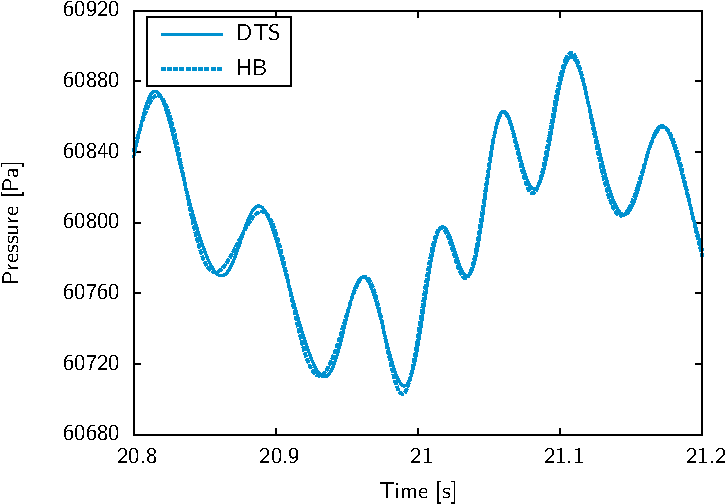
\includegraphics[width=.4\textwidth]{CANAL2_VALIDATION_HBT_GEAR_TIME_EV_PROBE_1_PPT.pdf}}
   \quad\subfigure[probe
   2]{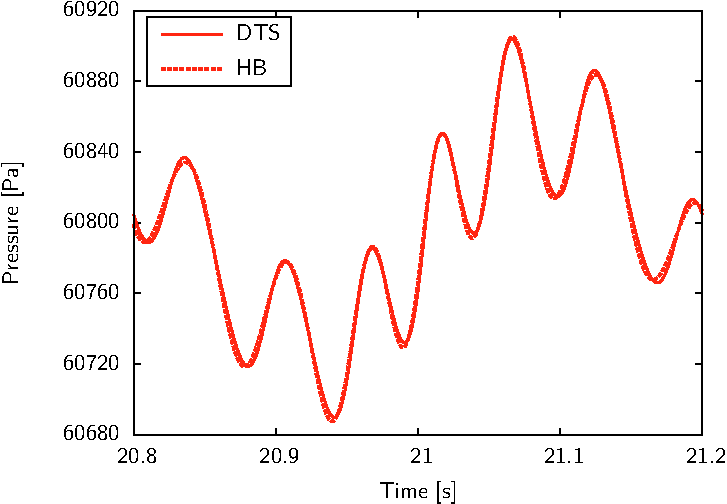
\includegraphics[width=.4\textwidth]{CANAL2_VALIDATION_HBT_GEAR_TIME_EV_PROBE_2_PPT.pdf}}
   \subfigure[probe
   3]{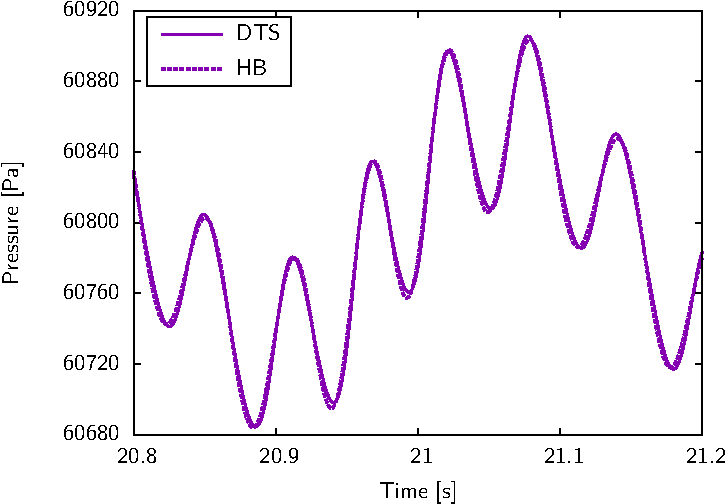
\includegraphics[width=.4\textwidth]{CANAL2_VALIDATION_HBT_GEAR_TIME_EV_PROBE_3_PPT.pdf}}
  \caption{Unsteady pressure signals at different axial positions.}
  \label{fig:canal2_validation_hbt_gear_time_ev}
\end{figure}


\chconclu{The mono- and multi-frequential harmonic balance
approaches have been validated in this chapter against selected
test problems. 
If the provided number of harmonics is greater than
a threshold value depending on the specif configuration, the solution is
superimposed to the exact/reference solution for both linear
and non-linear test cases. This property is called spectral accuracy.
In addition to that, it is shown that the multi-frequential harmonic
balance approach is a good candidate for the simulation of problems
involving segregated frequencies. Actually, this is the case
of contra-rotating open rotor aeroelasticity. In the following chapter,
we will see that an issue rises when considering segregated frequencies
with the multi-frequential harmonic balance approach. As this is likely
to be the case for contra-rotating open rotor aeroelasticity, an original
approach is proposed to alleviate this problem.}
